% !TEX root = ../thesis.tex

% set counter to n-1:
\setcounter{chapter}{2}

\chapter{Setup}\label{ch:setup}
This chapter describes how the different elements of the setup are brought together, how  the camera was calibrated and with which approach the two coordination systems of the UWB system and the one of the camera were matched together and with the help of which frameworks the steps were done.

In the second part of this chapter, the ROS setup (ROS nodes and messages) which was used is described. 

\section{Camera calibration}
As it is well known, that cameras, as the one used in this semester project, suffer from distortion (radial as well as tangential) \cite{Szeliski:2010:CVA:1941882}, \cite{opencv_library}, the required constants to remove this distortions as well as the camera matrix, needed for the unit conversion, are determined by the camera calibration.

In this semester project, the camera calibration framework of the OpenCV library \cite{opencv_library} was used, as it is easy to handle and well known to work properly.

\section{UWB and camera mounting}
The UWB system and the camera are mounted in a way, that the center of their relative coordination systems have a fixed, not too large displacement. This setup is shown in \autoref{fig:setup}. In this setup, the origin of the camera coordination system is a bit above of the one from the UWB system (indicated by the blue arrow in \autoref{fig:setup}), which is positioned in the middle of the monitor screen. 

\begin{figure}[h]\centering
	\includegraphics[width=0.5\textwidth]{figures/Monitor_cut.jpg}
	\caption{UWB and camera setup.}\label{fig:setup}
\end{figure}

\section{Matching frames}
The coordination systems of the UWB setup and the one of the camera are not the same, as sketched in \autoref{fig:coordinationsystem}. As the goal of this semester project is to fuse the locations provided by the UWB system and by the vision tracker, the locations must be transformed from one to the other. To achieve this, the location of the object in 3D must be available from both systems (UWB and vision).

For the vision system, the ArUco \cite{Aruco2014} library and an ArUco marker were used to get the 3D coordinates of the object, as explained in \autoref{subsec:aruco}.

The translation as well as the rotation between the two coordination systems were then determined by the Kabsch algorithm \cite{Kabsch:a12999} in the matching proceeder, explained in \autoref{subsec:matching}.
\begin{figure}[ht!]\centering
	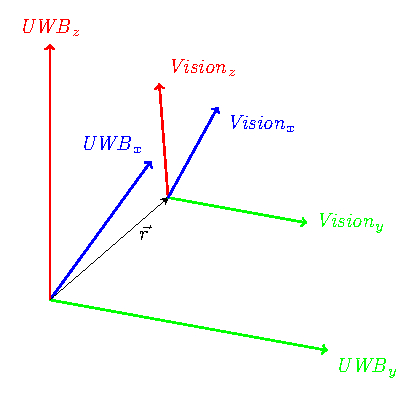
\includegraphics[width=0.5\textwidth]{figures/coordination_system}
	\caption{The two coordination systems relative to each other.}\label{fig:coordinationsystem}
\end{figure}

\subsection{ArUco}\label{subsec:aruco}
ArUco \cite{Aruco2014} presents itself as a minimal library for augmented reality applications based on OpenCV. ArUco is a marker system specialized for camera pose estimation in different applications such as augmented reality, robot localization, etc. ArUco contains an algorithm for the generation of markers as well as marker boards and an algorithm for the automatic detection of markers. A third contribution of ArUco is a solution to the occlusion problem in augmented reality applications which is not of interest for this semester project.

To get 3D vision coordinates, an ArUco marker was mounted on the object, as shown in \autoref{fig:target}, right in front of an UWB target and an application was written which uses the ArUco library to read out the 3D coordination of detected ArUco markers and saves them for the later usage by the matching proceeder.
\begin{figure}[ht!]\centering
	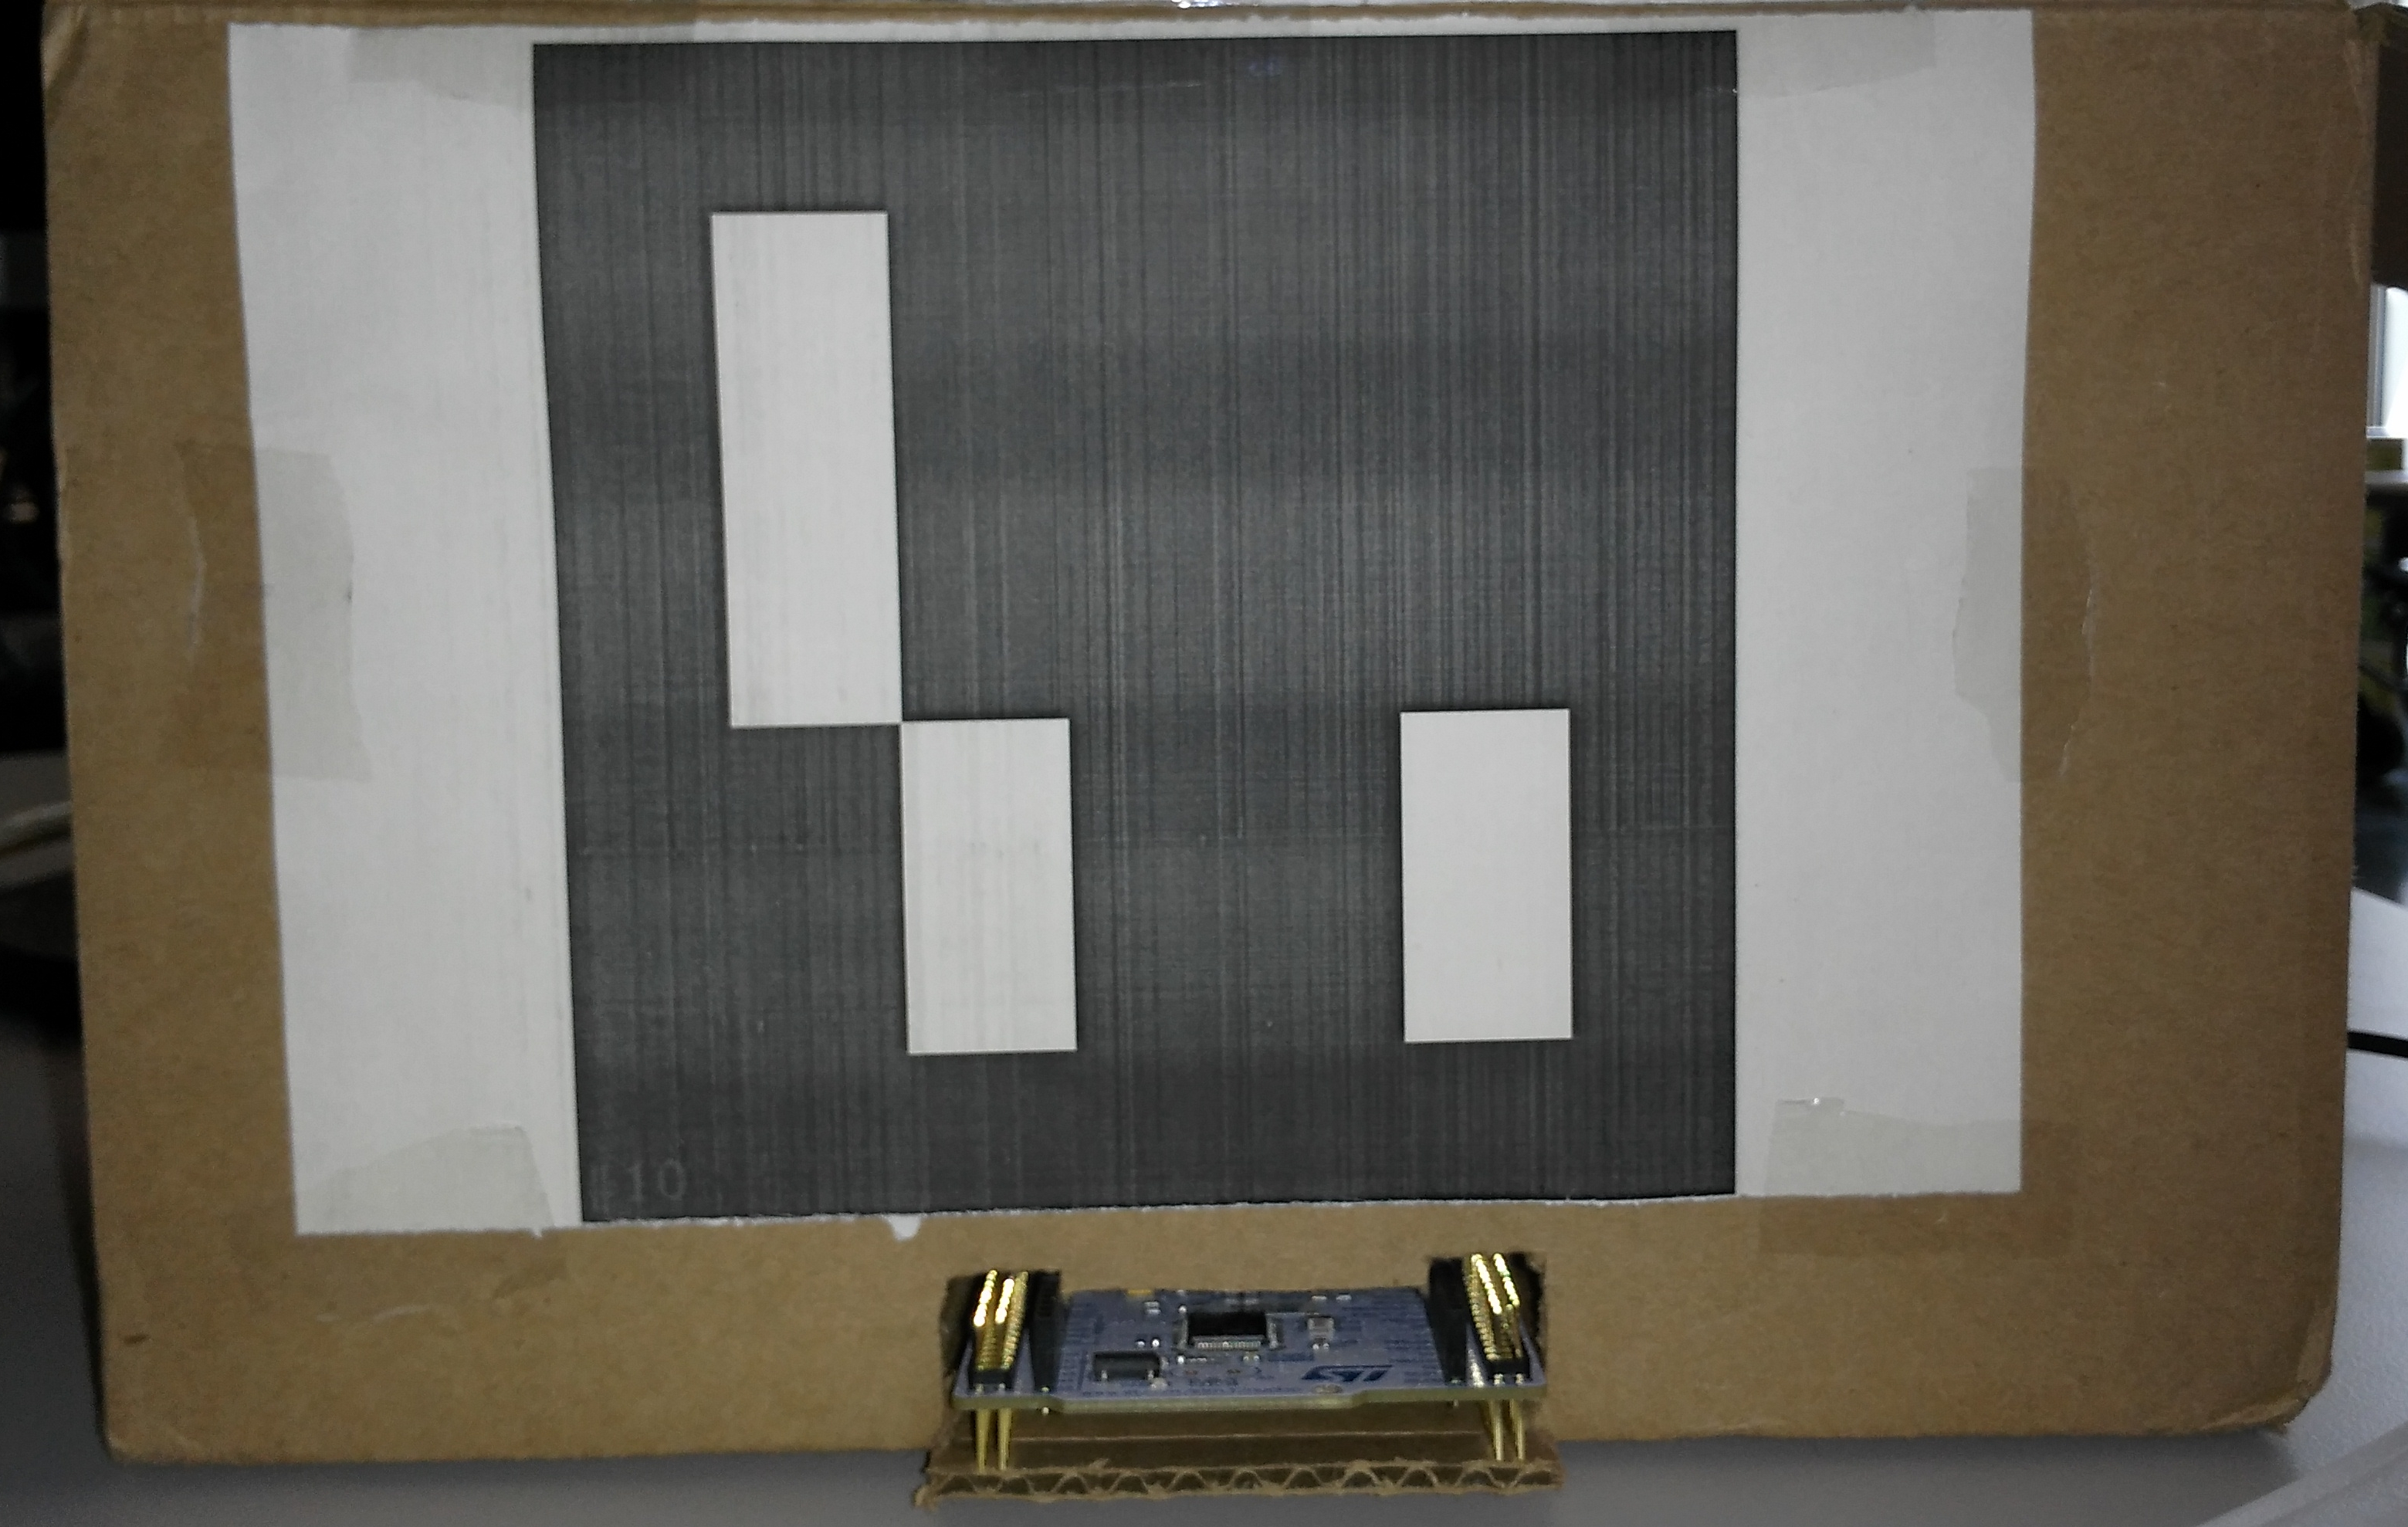
\includegraphics[width=0.5\textwidth]{figures/Box_cut.jpg}
	\caption{ArUco marker and UWB target.}\label{fig:target}
\end{figure}

\subsection{Kabsch}
The Kabsch algorithm \cite{Kabsch:a12999} calculates the optimal rotation matrix and translation vector that minimizes the root mean squared deviation between two paired sets of points. In this semester project, the Kabsch algorithm determines the optimal rotation matrix and translation vector between the coordination systems of the UWB system an the one of the camera.

\subsection{Matching proceeder}\label{subsec:matching}
For the matching proceeder, a Matlab script was written, shown in \autoref{lst:matching}, which calculates the mean of the UWB and the vision (ArUco) coordinates, centralizes the coordinates of both, calculates the scale from the centralized coordinates, scales the vision (ArUco) coordinates and finally executes the Kabsch algorithm to calculate the rotation matrix $\textbf{U}$, the translation $\vec r$ and the least root mean squared error $\text{lrms}$.

The determined rotation matrix $\textbf{U}$ and the translation vector $\vec r$ applied on a set of measured points by the UWB systems together with the set of measured points by ArUco results in a data set as shown in \autoref{fig:matching}

\lstset{language=Matlab}
\begin{lstlisting}[frame=single, caption=Matching proceeder, label=lst:matching]
% Calculate mean
mean_uwb = mean(uwb(1:3,:), 2);
mean_aruco = mean(aruco(1:3,:), 2);
	
% normalize data	
aruco_centred(1,:) = (aruco(1,:) - ...
		mean_aruco(1)*ones(1,length(aruco(1,:))));
aruco_centred(2,:) = (aruco(2,:) - ...
		mean_aruco(2)*ones(1,length(aruco(1,:))));
aruco_centred(3,:) = (aruco(3,:) - ...
		mean_aruco(3)*ones(1,length(aruco(1,:))));

uwb_centred(1,:) = uwb(1,:) - ...
		mean_uwb(1)*ones(1,length(uwb(1,:)));
uwb_centred(2,:) = uwb(2,:) - ...
		mean_uwb(2)*ones(1,length(uwb(2,:)));
uwb_centred(3,:) = uwb(3,:) - ...
		mean_uwb(3)*ones(1,length(uwb(3,:)));
	
% calculate scale
scale = norm(uwb_centred)/norm(aruco_centred);
	
aruco = scale .* aruco;
	
	
[U, r, lrms] = Kabsch(aruco, uwb);
\end{lstlisting}

\begin{figure}[ht!]\centering
	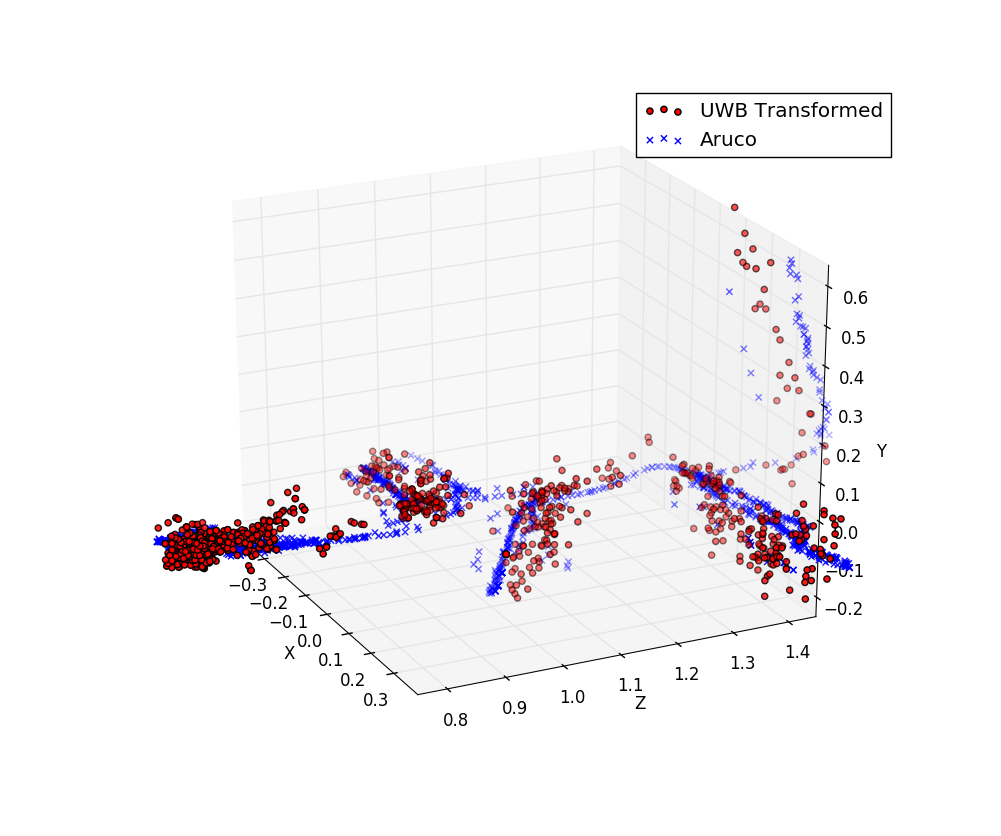
\includegraphics[width=1.0\textwidth]{figures/matching}
	\caption{Matching of the position set of ArUco and UWB.}\label{fig:matching}
\end{figure} 

\section{ROS setup}
In this semester project three different ROS setups were used to perform the tasks of recording the video from the camera as well as recording the measurements from the UWB system, collecting the data required for the matching proceeder and for the object tracking task.

The first setup to record the video and the measurement of the UWB system is described in \autoref{subsec:recording}.

The setup to gain the required data to perform the matching proceeder explained in \autoref{subsec:matching}, is described in \autoref{subsec:kabsch}.

The third and last ROS setup that was used in this semester project, is the setup introduced in \autoref{subsec:tracking}, which is used for the main task, the object tracking.

\subsection{Recording setup}\label{subsec:recording}
In the recording setup, shown in \autoref{fig:recording}, a rosbag node records the messages from the two nodes publish\_image and uwb. The message "/camera/video" from the publish\_image node is the image stream from the camera. The node uwb sends the message "/uwb/tracker" which consists of the position and the velocity of the target as well as their covariances.

\begin{figure}[h]\centering
	\includegraphics[width=0.8\textwidth]{figures/blockdiagram_recording}
	\caption{Block diagram of the ROS nodes and messages for the recording setup.}\label{fig:recording}
\end{figure}

\subsection{Kabsch setup}\label{subsec:kabsch}
To save the required data to perform the matching proceeder described in \autoref{subsec:matching}, the setup, shown in \autoref{fig:kabsch}, was used. In this ROS setup the node uwb\_aruco receives the messages "/camera/video" and "/uwb/tracker". It saves the positions measured by the UWB system directly and performs the ArUco marker detection to get the positions detected by ArUco and also saves them.

\begin{figure}[h]\centering
	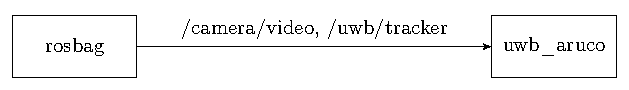
\includegraphics[width=0.8\textwidth]{figures/blockdiagram_kabsch}
	\caption{Block diagram of the ROS nodes and messages for the Kabsch setup.}\label{fig:kabsch}
\end{figure}

\subsection{Tracking setup}\label{subsec:tracking}
This ROS setup, shown in \autoref{fig:tracking}, is used for the main task, the object tracking. In this setup, the node vision\_tracker performs the object tracking on the images it receives from the node rosbag in the messages "/camera/video". It then publishes the position of the tracked object in the messages "/vision\_tracker/vision\_coordinates". The node fusing receives the positions measured by the UWB system in the messages "/uwb/tracker" as well as the positions of the object detected by the node vision\_tracker in the messages "/vision\_tracker/vision\_coordinates. With an Extended Kalman Filter (EKF), described in \autoref{ch:fusing}, the node fusing estimates the position of the tracked object.

\begin{figure}[h]\centering
	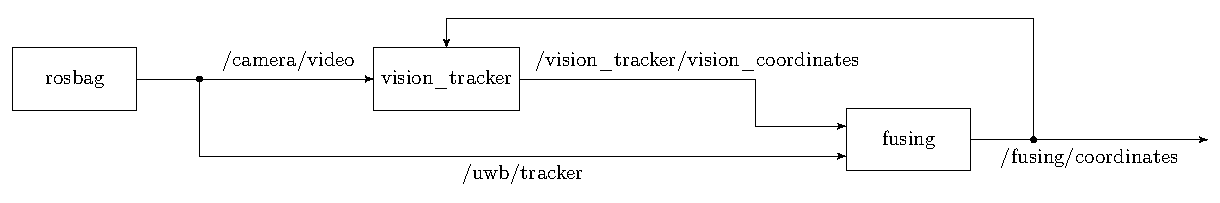
\includegraphics[width=1.0\textwidth]{figures/blockdiagram_tracking}
	\caption{Block diagram of the ROS nodes and messages for the tracking setup.}\label{fig:tracking}
\end{figure}
